\chapter{VarBench: variational benchmarks for quantum many-body systems}
\label{ch:varbench}

The previous chapters have introduced multiple variational methods for quantum many-body systems, including variational Monte Carlo (VMC) in \cref{ch:vmc} and tensor networks (TNs) in \cref{ch:tn}, each with its own appropriate use cases, as well as trade-off between accuracy and computational cost. When different methods are applied to the same physical system, there is a simple criterion to assess their performance: A lower variational energy indicates that the method approximates the true ground state more accurately. Besides that, it is also attempting to compare the accuracies of one method on different physical systems, or compare the universal applicability of two methods on multiple systems. Therefore, we require a metric that can be compared both between methods and between systems.

In the following, we present the metric proposed in Ref.~\cite{wu2024variational}, namely V-score. It is used in the VarBench project, an extensive collection of benchmarks for the accuracies of variational methods on a diverse variety of quantum many-body systems. Moreover, the V-score can measure the hardness of simulating a physical system, which identifies certain hard systems that are not yet solved by available computational techniques.

\section{V-score: universal metric for variational accuracy}

It has been widely observed that when a variational state is sufficiently close to the ground state, the variance of the variational energy $\Var E = \ev{\hat{H}^2} - \ev{\hat{H}}^2$ scales linearly with the difference between the variational energy $E$ and the ground state energy $E_0$~\cite{kwon1993, imada2000, sorella2001}:
\begin{equation}
E  - E_0 = A \Var E + O\left( (\Var E)^2 \right),
\label{eq:var-linear}
\end{equation}
where $A$ is a coefficient depending on the properties of the Hamiltonian $\hat{H}$ and the variational state $\ket{\psi}$. For example, in a simple two-state system as discussed in \cref{eq:var-two-states}, we have
\begin{equation}
A = \frac{1}{E_1 - E_0}.
\end{equation}
For general systems with more energy levels, Ref.~\cite{taddei2015iterative} has given more rigorous conditions of ``sufficiently close'' to hold \cref{eq:var-linear}, which are usually satisfied in computational studies. It has been common practice to linearly extrapolate $E$ as a function of $\Var E$ and obtain an estimation of $E_0$ at $\Var E = 0$. Therefore, even though we do not know the true ground state $E_0$, the variance can indicate the accuracy of approximating the given Hamiltonian, and we seek a metric proportional to it.

The metric should be a dimensionless number, so we normalize the variance by the variational energy and obtain $\frac{\Var E}{E^2}$. Moreover, it should not scale with the system size $N$. The energy $E$ scales linearly with $N$, as it is an extensive quantity for all physical systems of our interest. The variance $\Var E$ also scales linearly with $N$ if the Hamiltonian satisfies the following clustering property~\cite{park1995uniqueness, nachtergaele2006lieb, hastings2006spectral}: The Hamiltonian can be written as a sum of $N$ terms labeled by the site index $i$,
\begin{equation}
\hat{H} = \sum_{i = 1}^N \hat{h}_i,
\end{equation}
and the correlations between these terms decay quickly enough with the spatial distance of the sites,
\begin{equation}
\left| \ev*{\hat{h}_i \hat{h}_j} - \ev*{\hat{h}_i}\!\ev*{\hat{h}_j} \right| \le \frac{A_\text{corr}}{d^{D + \epsilon}(i, j)},
\end{equation}
where $A_\text{corr}$ is a constant for all $i, j$, $d(i, j)$ is the distance between the sites $i, j$, $D$ is the spatial dimension, and $\epsilon$ is a small positive number for all $i, j$. All physical systems of our interest have this clustering property, and we note that for non-critical systems the correlations decay exponentially with the distance. Therefore, we scale the variance by $N$ and obtain $\frac{N\,\Var E}{E^2}$, which is asymptotically independent of $N$.

The remaining issue is that we can arbitrarily shift the Hamiltonian by a constant: $\hat{H} \gets \hat{H} + C$, which does not change any physical property of the system, and our metric should be invariant under this shift. To achieve this, we define a zero point of energy $E_\infty$, and replace $E$ by $E - E_\infty$. For spin and fermionic systems with a finite number of energy levels per site, $E_\infty$ is defined to be the expected energy of a random state in the Hilbert space, and we are sure that a variational state after optimization typically has a lower energy than a random state. It is equivalent to the expected energy of a thermal state at infinite temperature, which can be derived from the trace of the Hamiltonian:
\begin{equation}
E_\infty = \frac{\tr \hat{H}}{\dim \calH},
\label{eq:E-infty-trace}
\end{equation}
where $\dim \calH$ is the dimension of the Hilbert, or the Hilbert subspace for fermionic systems when the number of fermions is fixed. It can be analytically derived for simple Hamiltonians or numerically evaluated using Monte Carlo sampling. However, it remains an open question to define $E_\infty$ for bosonic systems because there are infinitely many energy levels per site. We may define it with a cutoff of physically relevant energy levels or a mean-field energy, but there is not yet an intuitive definition that is consistent with spin and fermionic systems.

The resulting definition of the metric for variational accuracy, namely V-score, is
\begin{equation}
\text{V-score} = \frac{N\,\Var E}{(E - E_\infty)^2}.
\label{eq:v-score}
\end{equation}
It is dimensionless, asymptotically independent of the system size, and invariant to the energy shift. Moreover, it can be efficiently evaluated without knowing the ground state energy. Substituting \cref{eq:var-linear,eq:v-score} into the energy relative error $\frac{E - E_0}{|E_0 - E_\infty|}$, we can obtain the linear relation
\begin{align}
\frac{E - E_0}{|E_0 - E_\infty|} &= B\,\text{V-score} + O(\text{V-score}^2), \label{eq:v-score-rel-err} \\
B &= \frac{A (E - E_\infty)^2}{N |E_0 - E_\infty|},
\end{align}
where $A$ has the dimension of $E^{-1}$ and is asymptotically independent of $N$. For any Hamiltonian with the clustering property and any variational state converging to the ground state, the magnitude of $B$ will not be far from $1$. Therefore, the V-score can be a universal metric to predict the energy relative error in variational approximation, which will be visualized in \cref{fig:v-score-rel-err}.

It is worth discussing the possibilities for the V-score to underestimate or overestimate the energy relative error. An intuitive case of the underestimation is when the variational state converges to an excited state, as $\Var E$ under any excited state is zero. This situation can be detected by applying the symmetries of the ground state or repeating the optimization with different initial parameters. Another case is the mode collapse discussed in \cref{sec:vmc-var}, where we estimate $\Var E$ using $|E_\text{loc}(\vs)|^2$, and it can be detected by actually evaluating the matrix elements of $\hat{H}^2$.

If the V-score overestimates the energy relative error, an upper bound of their ratio is proven that
\begin{equation}
\frac{\text{V-score}}{(E - E_0) / (E_\infty - E_0)} \le N \frac{(E_\infty - E_0) (E_\text{M} - E)}{(E_\infty - E)^2},
\label{eq:v-score-bound}
\end{equation}
where $E_\text{M}$ is the highest energy level of the system, and the variational state can be an arbitrary linear combination of the eigenstates. This is a loose upper bound as it scales linearly with $N$, and it remains an open question to find a tighter upper bound under more assumptions, such as the variational state being close to the ground state.

\section{Hamiltonians and variational methods in the benchmark}

To demonstrate the universal applicability of V-score, in the VarBench project we have collected more than $400$ numerical studies with many kinds of variational methods on spin and fermionic Hamiltonians. The Hamiltonians mainly include the following:
\begin{enumerate}
\setlength{\itemsep}{0ex}
\item The spin-$\frac{1}{2}$ transverse-field Ising model (TFIM)
\begin{equation}
\hat{H} = J \sum_{\langle i, j \rangle} \hat{\sigma}^z_i \hat{\sigma}^z_j
+ \Gamma \sum_i \hat{\sigma}^x_i,
\tag{\ref{eq:qu-ising}}
\end{equation}
where $\langle i, j \rangle$ runs over nearest neighbors, $\Gamma$ is the transverse field strength, $\hat{\sigma}^x, \hat{\sigma}^y, \hat{\sigma}^z$ are the Pauli matrices, and we always set $J = 1$.

\item The spin-$\frac{1}{2}$ Heisenberg model
\begin{equation}
\hat{H} = J \sum_{\langle i, j \rangle} \hat{\vsi}_i \cdot \hat{\vsi}_j,
\tag{\ref{eq:heis}}
\end{equation}
where $\hat{\vsi}_i \cdot \hat{\vsi}_j = \hat{\sigma}^x_i \hat{\sigma}^x_j + \hat{\sigma}^y_i \hat{\sigma}^y_j + \hat{\sigma}^z_i \hat{\sigma}^z_j$.

\item The spin-$\frac{1}{2}$ $J_1$-$J_2$ model
\begin{equation}
\hat{H} = J_1 \sum_{\langle i, j \rangle} \hat{\vsi}_i \cdot \hat{\vsi}_j
+ J_2 \sum_{\llangle i, j \rrangle} \hat{\vsi}_i \cdot \hat{\vsi}_j,
\end{equation}
where $\llangle i, j \rrangle$ runs over next-nearest neighbors (diagonals if the lattice is a 2D grid), $J_2$ is the next-nearest neighbor interaction strength, and we always set $J_1 = 1$.

\item The spinless fermionic $t$-$V$ model
\begin{equation}
\hat{H} = -t \sum_{\langle i, j \rangle} \left( \hat{c}^\dagger_i \hat{c}_j + \hat{c}^\dagger_j \hat{c}_i \right)
+ V \sum_{\langle i, j \rangle} \hat{n}_i \hat{n}_j,
\end{equation}
where $V$ is the Coulomb repulsive interaction strength, $\hat{c}^\dagger_i$ and $\hat{c}_i$ are the fermionic creation and annihilation operators respectively, $\hat{n}_i = \hat{c}^\dagger_i \hat{c}_i$ is the number operator, the number of fermions is fixed to $N_\text{f}$, and we always set $t = 1$.

\item The spin-$\frac{1}{2}$ fermionic Hubbard model
\begin{equation}
\hat{H} = -t \sum_{\langle i, j \rangle, \sigma} \left( \hat{c}^\dagger_{i \sigma} \hat{c}_{j \sigma} + \hat{c}^\dagger_{j \sigma} \hat{c}_{i \sigma} \right)
+ U \sum_i \hat{n}_{i \spinup} \hat{n}_{i \spindown},
\end{equation}
where $U$ is the on-site interaction strength, the numbers of fermions are fixed to $N_\spinup$ and $N_\spindown$, and we only consider the case of $N_\spinup = N_\spindown$.
\end{enumerate}
These Hamiltonians can be defined on all kinds of lattice geometries, including the non-frustrated 1D chains and 2D grids, the frustrated 2D triangular~\cite{li2015rare, liu2020intrinsic}, kagome~\cite{norman2016colloquium}, and shuriken~\cite{siddharthan2001square, astrakhantsev2021pinwheel} lattices, as well as 3D pyrochlore lattices~\cite{moessner1998properties, astrakhantsev2021broken}. The boundary conditions of these lattices also affect the results. In addition, we include Anderson impurity models, which have applications in fields such as quantum embedding and nanoelectronic devices~\cite{anderson1961localized, kanamori1963electron, lu2019natural, cao2021tree, cao2024vision}.

The variational methods benchmarked are categorized by:
\begin{enumerate}
\setlength{\itemsep}{0ex}
\item VMC with physically motivated ansatzes (PMAs) in \cref{sec:jastrow,sec:gutz}.
\item VMC with neural quantum states (NQSs) in \cref{sec:nqs}.
\item TNs in \cref{ch:tn}, most of which are matrix product states (MPSs) optimized using the density matrix renormalization group (DMRG).
\item Parameterized quantum circuits (PQCs)~\cite{cerezo2021variational, wecker2015progress} optimized using variational quantum eigensolver (VQE)~\cite{peruzzo2014variational, seki2020symmetry, astrakhantsev2023phenomenological}.
\item Variational auxiliary-field quantum Monte Carlo (VAFQMC)~\cite{sorella2021phase} for the Hubbard model.
\end{enumerate}

An overview of the complete benchmark results is visualized in \cref{fig:v-score}.

\newpage

\begin{figure}[!h]
\centering
\hspace*{-0.05\linewidth}
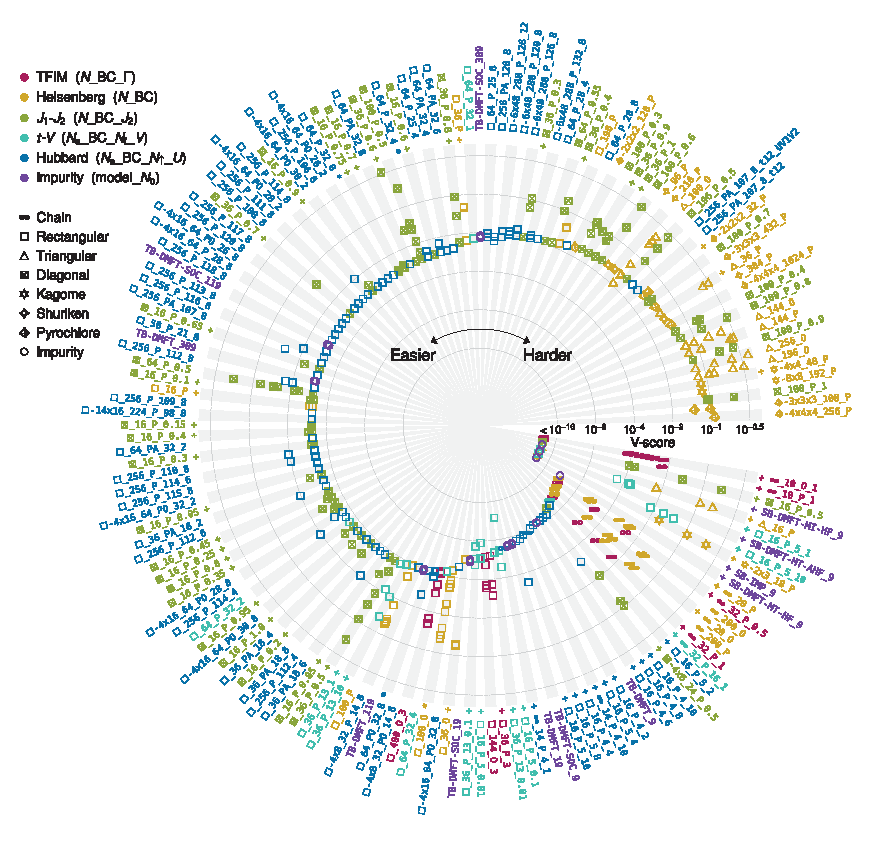
\includegraphics[width=1.05\linewidth]{ch10/v_score_polar_doubly_log.pdf}
\caption[Overview of VarBench results]{
Overview of the complete benchmark results.
Each slice in the radial direction contains different variational methods for a given Hamiltonian. The bold marker indicates the method with the lowest variational energy (rather than the lowest V-score), which defines the V-score for the Hamiltonian and determines its clockwise ranking.
The radial axis uses the doubly log scale to show the results across a wide range of V-score magnitude.
The results with V-scores less than $10^{-16}$ are indistinguishable from the exact solutions due to limited numerical precision.
The label outside each slice is the name of the Hamiltonian in the dataset, which describes the lattice geometry, the lattice size $N_\text{s}$, the boundary conditions (BC), and the Hamiltonian parameters such as the interaction strength ($\Gamma$, $J_2$, $V$, $U$) and the number of particles ($N_\mathrm{f}$, $N_{\uparrow}$, $N_\mathrm{b}$).
The BC can be O (open), P (periodic), A (anti-periodic) on each dimension.
The `\texttt{+}' marker near the label indicates that an ED solution is available for that Hamiltonian, and the `\texttt{\textasteriskcentered}' marker indicates a numerically exact QMC solution.
This figure is reproduced from Fig.~3 in Ref.~\cite{wu2024variational}.
}
\label{fig:v-score}
\end{figure}

\newpage

\section{Benchmark results}

\begin{figure}[htb]
\centering
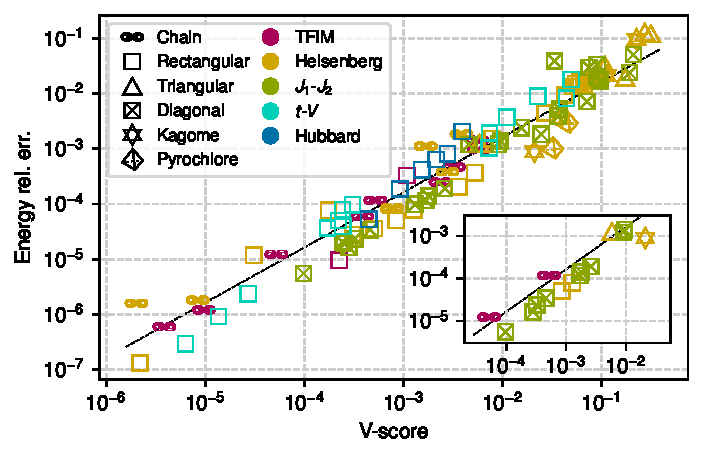
\includegraphics[width=0.75\linewidth]{ch10/v_score_rel_err.pdf}
\caption[Comparison of V-score and energy relative error]{
Comparison of V-score and energy relative error for systems whose exact solutions from ED or QMC are available.
The black dashed line is fitted by least-squares regression with the slope fixed to $1$.
The inset focuses on PQC results simulated on classical hardware without noise.
This figure is reproduced from Fig.~2 in Ref.~\cite{wu2024variational}.
}
\label{fig:v-score-rel-err}
\end{figure}

We first compare the V-scores with the known energy relative errors, for small systems whose ground state energies are obtained by exact diagonalization (ED), and simple systems for which quantum Monte Carlo (QMC) methods produce numerically exact results. As shown in \cref{fig:v-score-rel-err}, the results in the log-log plot can be fitted with high confidence using least-squares regression where the slope is fixed at $1$. This validates their linear relation in \cref{eq:v-score-rel-err}, where the magnitude of the coefficient $B$ does not change substantially between Hamiltonians and variational methods. Therefore, we can use the V-score to predict the energy relative error, at least up to the order of magnitude, for systems whose ground state energies cannot be practically obtained in other ways.

\begin{figure}[htb]
\centering
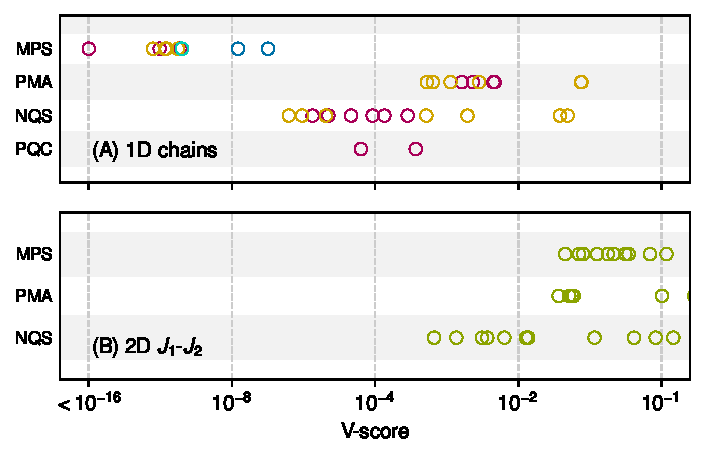
\includegraphics[width=0.75\linewidth]{ch10/v_score_method_doubly_log.pdf}
\caption[V-scores of different variational methods]{
V-scores of different variational methods, including matrix product state (MPS), physically motivated ansatz (PMA), neural quantum state (NQS), and parameterized quantum circuit (PQC), for (a) all Hamiltonians on 1D chains and (b) the $J_1$-$J_2$ model on 2D grids.
The $x$-axis uses the doubly log scale to show the results across a wide range of V-score magnitude.
}
\label{fig:v-score-method}
\end{figure}

Then we select some Hamiltonians of interest and compare different kinds of variational method on them. It is generally agreed that for 1D systems, MPSs can solve them with high accuracy, and the more complicated NQSs and PQCs are unnecessary, which is shown in \cref{fig:v-score-method}~(a). In contrast, for the 2D $J_1$-$J_2$ model with frustrated interactions, especially in the supposed spin liquid phase~\cite{dagotto1989phase, schulz1996magnetic, hu2013direct, liang2018solving, liu2018gapless, choo2019two, nomura2021dirac}, the most accurate records are produced by NQSs. Therefore, the V-score can clearly demonstrate the appropriate use cases of different variational methods.

\section{Hardness of Hamiltonian}

\begin{figure}[htb]
\centering
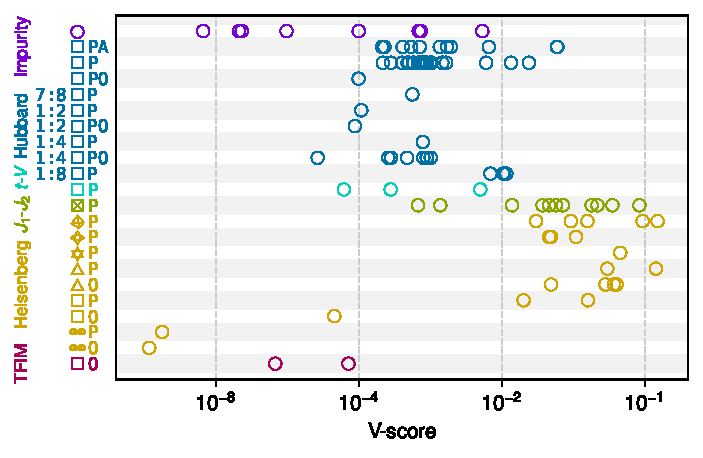
\includegraphics[width=0.75\linewidth]{ch10/v_score_ham_no_ed_doubly_log.pdf}
\caption[V-scores of different Hamiltonians]{
V-scores of different Hamiltonians, classified by Hamiltonian types and lattice geometries.
Only the Hamiltonians without ED results are shown.
The $x$-axis uses the doubly log scale to show the results across a wide range of V-score magnitude.
The ratios to the left of the lattice icons are aspect ratios of rectangular lattices. The letters to the right are boundary conditions, which can be O (open), P (periodic), A (anti-periodic) on each dimension.
This figure is reproduced from Fig.~4 in Ref.~\cite{wu2024variational}.
}
\label{fig:v-score-ham}
\end{figure}

The V-score can assess not only the accuracy of any variational method but also the hardness to simulate any Hamiltonian. If we have applied all available methods but still cannot obtain a low V-score, then we consider the Hamiltonian to be hard, so the V-score of the best method (with the lowest variational energy, rather than the lowest V-score) is practically defined to be the V-score of the Hamiltonian.

The V-scores of the Hamiltonians benchmarked are plotted in \cref{fig:v-score-ham}. The easy Hamiltonians include the stoquastic Ising and Heisenberg models on the non-frustrated chains and grids, as well as small-sized systems, which are already well solved with V-scores lower than $10^{-4}$. In contrast, the hard Hamiltonians include the non-stoquastic $J_1$-$J_2$ and Hubbard models, as well as the frustrated lattices, whose V-scores remain higher than $10^{-2}$.

These hard Hamiltonians can serve as the aims for the development of more advanced computational methods, particularly quantum computers. In quantum computing theory, random circuit sampling~\cite{lund2017quantum, boixo2018characterizing, arute2019quantum} is a traditional task to demonstrate the quantum advantage, but currently developed quantum computing platforms actually do not outperform large-scale classical computers on this task~\cite{pan2022solving, aharonov2023polynomial, gao2024limitations, zhao2024leapfrogging}. Meanwhile, the demonstration of quantum advantage on tasks with more practical impact is still under active research~\cite{daley2022practical}. The hard Hamiltonians identified by the V-score are exactly a kind of tasks promising for quantum computers to solve~\cite{feynman1982simulating}, with practical impact in physics.

In the inset of \cref{fig:v-score-rel-err}, we provide the initial insights of small-scale PQCs simulated on classical hardware without noise, where their V-scores reliably predict their energy relative errors. While larger-scale simulations of PQCs and noisy intermediate-scale quantum (NISQ) platforms are in active development, the V-score will be a useful metric to track their progress.

\section{Conclusion}

In conclusion, the V-score is a universal metric for the accuracy of variational approximation, which can be compared both between variational methods and between Hamiltonians. It also measures the hardness of simulating any Hamiltonian and identifies the hard ones that are not yet solved by any available method. These Hamiltonians are the targets for the future development of computational methods, especially the demonstration of quantum advantage. The generalization of the V-score to bosonic and molecular systems is still under investigation, which would further extend its universality. It would also be interesting to study the behavior of the V-score with the change of Hamiltonian parameters such as $J_2$, and possibly discover some universal critical exponents.

The VarBench project is an extensive collection of benchmarks for many kinds of variational methods and quantum many-body systems. Besides witnessing the previous development of methods, it also provides a framework to test new methods on a collection of Hamiltonians, which helps to thoroughly and orthogonally assess their performance. We plan to continuously update it with the development of new methods and computational power, especially experimental results of quantum computing platforms, and possibly set up a website like PubChem and PapersWithCode to ease the collaboration of the community. A topic not covered by the VarBench project is the computational costs of all these methods, and it would be another huge challenge to systematically measure them and quantify their relation to the accuracies of the methods.
